\documentclass[a4paper,10pt]{article}
\setlength{\parindent}{0ex}
\setlength{\parskip}{1.5ex}
\usepackage[dvips]{graphicx}
\usepackage {epsfig}
\usepackage[a4paper, hmargin=25mm, vmargin=20mm, nohead]{geometry}

\begin{document}
\newcommand{\marks}[1]
{\begin{flushright}{\bf (#1 marks)}\end{flushright}}

{\centering \large \bf THE UNIVERSITY OF WAIKATO\\}
{\centering \large \bf Department of Computer Science\\[0.5cm]}

{\centering \large \bf COMP201Y Computer Systems 2004\\}
{\centering \large \bf Exercise 6 Test - 2nd August 2004\\[0.3cm]}
{\centering \bf Worth 7\% --- Marked out of: 30\\[0.3cm]}
{\centering \bf Time allowed: 45 Min\\[1cm]}
\hrule

\begin{enumerate}
\item True/False answers. Indicate on your answer sheet if the
following statements are true or false.

\begin{enumerate}

\item When setting up exceptions, the address of your exception
handler should be loaded into the Exception Address Register
(\texttt{\$ear})

\item Software exceptions can be disabled on the WRAMP processor.

\item Interrupts are disabled when an exception occurs.

\item When an exception occurs the cause can be determined by
examining the Exception Status Register (\texttt{\$estat})

\item If an interrupt is not acknowledged then it will not occur again
until it is acknowledged.

\end{enumerate}

\marks{5}

\item State two main effects the \texttt{'rfe'} instruction has when
executed. In particular state any special registers that this
instruction changes, or uses.

\marks{3}

\item Examine the code provided in Figure~\ref{code:timer} that sets
up the Timer. Using the specifications of the REX Timer device
provided in Appendix~\ref{appen:timer}, determine the delay between
timer interrupts (in seconds).

\marks{2}
\begin{figure}[h]
\begin{small}
\begin{center}
\begin{tabular}{|p{6cm}|}
\hline
\begin{verbatim}
  1:   sw    $0, 0x72003($0)
  2:   addi  $1, $0, 12000
  3:   sw    $1, 0x72001($0)
  4:   addi  $1, $0, 0x3
  5:   sw    $1, 0x72000($0)
\end{verbatim}
\\ \hline
\end{tabular}
\end{center}
\end{small}
\caption{Timer Setup Code}
\label{code:timer}
\end{figure}

\newpage
\item Provided in Figure~\ref{code:badack} is some code which should
use the REX board timer to provide an interrupt once per second. Each
time an interrupt occurs an \texttt{'X'} should be printed. When the code is
executed however, the program pauses for one second, and then
continuously displays \texttt{X}'s on the Terminal.

\label{ques:badack}

\begin{enumerate}
\item What is the error in the code that causes this problem ?
\marks{1}

\item Explain why this error results in the above behaviour.
\marks{2}

\item State the changes that you would make to ensure the code worked
as it should. You should provide the line numbers of any code that you
would change or the location that you would insert any new code into.
\marks{2}

\end{enumerate}

\begin{figure}[p]
\begin{footnotesize}
\begin{center}
\begin{tabular}{|p{12cm}|}
\hline
\begin{verbatim}
   1:  .text
   2:  .global main
   3:  main:
   4:    # Get the old exception vector
   5:    movsg  $2, $evec
   6:    # ...and save it.
   7:    sw     $2, old_vector($0)
   8:    # Get the address of my exception handler
   9:    la     $2, handler
  10:    # put it into the exception vector register
  11:    movgs  $evec, $2
  12:
  13:    # Get the CPU control register
  14:    movsg  $2, $cctrl
  15:    # Mask out all interrupts
  16:    andi   $2, $2, 0xf
  17:    # Enable IRQ2 (Timer) and Interrupt Enable.
  18:    ori    $2, $2, 0x42
  19:    # Replace the CPU control register
  20:    movgs  $cctrl, $2
  21:    
  22:    # Acknowledge any outstanding timer interrupts
  23:    sw     $0, 0x72003($0)
  24:    # Setup the delay between interrupts to 1 second.
  25:    addi   $2, $0, 2400
  26:    sw     $2, 0x72001($0)
  27:    # Setup the timer control register (AutoRestart and Timer Enable)
  28:    addi   $2, $0, 0x3
  29:    sw     $2, 0x72000($0)
  30:    
  31:  loop:   # Begin our main loop
  32:    # Read from the switches
  33:    lw     $2, 0x73000($0)
  34:    # Display the value on the SSDs
  35:    sw     $2, 0x73003($0)
  36:    srli   $2, $2, 4
  37:    sw     $2, 0x73002($0)
  38:    j      loop
  39:    
  40:  handler:
  41:    # Check the cause of the exception
  42:    movsg  $1, $estat
  43:    andi   $1, $1, 0xffb0
  44:    
  45:    # If timer then go to handle_interrupt
  46:    beqz   $1, handle_interrupt
  47:    
  48:    # Otherwise go to the system exception handler
  49:    lw     $1, old_vector($0)
  50:    jr     $1
  51:    
  52:  handle_interrupt:
  53:    # Check the serial status register
  54:    lw     $1, 0x71003($0)
  55:    # Check the transmit data sent bit
  56:    andi   $1, $1, 0x2
  57:    # Wait for the previous character to be sent
  58:    beqz   $1, handle_interrupt
  59:    # Send an 'X' to the terminal
  60:    addi   $1, $0, 'X'
  61:    sw     $1, 0x71000($0)
  62:    
  63:    # Return to the mainline
  64:    rfe
  65:
  66:  .data
  67:  old_vector:
  68:    .word  0
\end{verbatim}
\\ \hline
\end{tabular}
\end{center}
\end{footnotesize}
\caption{Code for Question~\ref{ques:badack}}
\label{code:badack}
\end{figure}

\item An alternative to printing 'X's on the timer interrupt is to use the
serial interrupt to detect input on the serial port connected to the Linux
machine.  Rewrite the setup code to enable these interrupts at the serial port
and the cpu.

\marks{5} 

\item The exception routine that you wrote for exercise 6 was not required to be
fully {\em compliant}.  In this context, what is meant by a fully compliant
exception handler?

\marks{3}

\newpage
\item Figure~\ref{code:handler} shows the code for the start of an
exception handler. This code is designed to distinguish between the
different sources of exceptions and decide which, of two handlers to
run.

The address of the previous exception handler routine was saved to the
memory location specified by the label \texttt{'old\_vector'} during
the initialisation phase of the program.

The provided code will transfer control either to the
\texttt{'my\_handler'} routine, or to the system exception handler
routine as specified by the address stored in the
\texttt{'old\_vector'} location.

For each of the possible exception sources given in
Table~\ref{table:esources} state which routine this code will transfer
control to if that exception had occurred. You should include all
working. The format of the \texttt{\$estat} register is provided in
Appendix~\ref{appen:estat}

\marks{5}

\begin{table}[h]
\begin{center}
\begin{tabular}{|l|l|}
\hline
IRQ0 & IRQ4, Serial Port 1 Interrupt \\
\hline
IRQ1, User Interrupt Button & IRQ5, Serial Port 2 Interrupt\\
\hline
IRQ2, Timer Interrupt & IRQ6 \\
\hline
IRQ3, Parallel Interrupt & IRQ7 \\
\hline
Arithmetic Exception & Breakpoint Exception \\
\hline
System Call Exception & General Protection Fault Exception \\
\hline
\end{tabular}
\end{center}
\caption{Exception sources for the WRAMP processor}
\label{table:esources}
\end{table}

\begin{figure}[h]
\begin{small}
\begin{center}
\begin{tabular}{|p{9cm}|}
\hline
\begin{verbatim}
   1:  handler:
   2:    # Get the exception status register
   3:    movsg  $1, $estat
   4:
   5:    andi   $1, $1, 0x7cb0
   6:
   7:    # If zero transfer control to my_handler
   8:    beqz   $1, my_handler
   9:
  10:    # Otherwise go to the system handler
  11:    lw     $1, old_vector($0)
  12:    jr     $1
  13:
  14:  my_handler:
  15:      . . . 	
\end{verbatim}
\\ \hline
% Will handle Arithmetic Exceptions, IRQ4, IRQ5, and IRQ2
\end{tabular}
\end{center}
\end{small}
\caption{Start of Exception Handler}
\label{code:handler}
\end{figure}
\end{enumerate}

\newpage
\appendix
\section{Programmable Timer}
\label{appen:timer}

The Programmable Timer on the REX board provides for generation of
interrupts at time intervals from about 1ms to 30s, with a resolution
of around 0.5ms.

The timer has an internal 16 bit register. This register is
decremented at a constant rate of 2400Hz. Once this register reaches
\texttt{0x0000} an interrupt is triggered. The starting value for the
timer is controlled by altering the value in the timer load register.

The timer can be configured to automatically reload the starting count
value and continue counting immediately after it expires.

The programmers view of the timer consists of four registers.  The
names of these registers and their addresses, expressed as offsets
from the base address, are provided in
Table~\ref{table:timer_offsets}.  The base address for the timer is
\texttt{0x72000}.

\begin{table}[h]
\begin{center}
\begin{tabular}{|l|c|}
\hline
\textbf{Register name} & \textbf{Offset} \\
\hline
Timer Control Register & 0 \\
\hline
Timer Load Register & 1 \\
\hline
Timer Count Register & 2 \\
\hline
Timer Interrupt Acknowledge Register & 3 \\
\hline
\end{tabular}
\caption{Timer Register Offsets}
\label{table:timer_offsets}
\end{center}
\end{table}


\subsection{Timer Control Register}

The Timer Control Register is a read/write register, that allows the
user to enable and control aspects of the timer operation. The timer
has two primary modes of operation, automatic restart and single-shot
mode. If the timer is set to automatic restart, as soon as the timer
expires, an interrupt is triggered and the timer immediately starts
counting down again. In single-shot mode the timer will copy the value
from the timer load register only once when the timer is enabled and
will count down to zero. Once the timer reaches zero an interrupt will
be triggered and the timer will be disabled.

\begin{figure}[h]
\begin{center}
\includegraphics[width=0.8\textwidth]{timer_cr.eps}
\caption{The Timer Control Register}
\label{timer_cr_pic}
\end{center}
\end{figure}

\subsection{Timer Load Register}

The Timer Load Register is a read/write register. This register allows
the user to specify the starting count value. The starting count value
is a 16 bit value with the upper 16 bits being ignored.

\subsection{Timer Count Register}

The Timer Count Register is a read-only register. Reading from this
register returns the current value in the 16 bit internal count
register.

\subsection{Timer Interrupt Acknowledge Register}

The Interrupt Acknowledge Register is a read/write register. This
register allows a program to detect a timer overrun as as well as
acknowledge interrupts that have been dealt with.

The overrun detected bit will be set if the timer is set to automatic
restart and the timer expired again before the previous interrupt was
acknowledged. This allows a program to detect if it is unable to
service the timer interrupt fast enough.

The overrun bit must be manually reset by writing a `\texttt{0}' to
it's location.

\begin{figure}[h]
\begin{center}
\includegraphics[width=0.8\textwidth]{timer_iack.eps}
\caption{The Timer Interrupt Acknowledge Register}
\label{timer_iack_pic}
\end{center}
\end{figure}

eg. If the value `\texttt{11}' was read from the interrupt acknowledge
register we could determine that the timer has overrun since we last
acknowledged an interrupt. If `\texttt{00}' was written to the timer
interrupt acknowledge register we will acknowledge any outstanding
interrupts and ensure the overrun bit is reset to zero.


\newpage
\section{\$cctrl - CPU Control Register}
\label{appen:cctrl}
\begin{figure}[h]
\begin{center}
\includegraphics[width=\textwidth]{cctrl.eps}
\caption{\$cctrl - CPU Control Register}
\label{cctrl_pic}
\end{center}
\end{figure}

The CPU control register controls almost all of the functionality
related to the WRAMP exception mechanism. There are three main
sections of this register:

\begin{itemize}
\item Interrupt Enable (IE)
\item Kernel/User Mode (KU)
\item Interrupt Mask
\end{itemize}

\subsection{Interrupt Enable}

This flag provides a global interrupt enable. If this location is set
to `\texttt{0}' then no interrupts can be triggered. This flag
\emph{only} affects external interrupts. There is no way on the WRAMP
processor to disable internal exceptions.

Interrupts that occur while the global interrupt enable is turned off
will be held back. As soon as interrupts are again enabled by writing
a `\texttt{1}' into this location the interrupt mask will be consulted
to discover if that specific interrupt is enabled. See
Section~\ref{sec:imask} for more information about the interrupt mask.

The CPU will automatically set the IE bit to `\texttt{0}' whenever an
exception of any type occurs. This prevents the exception handler
from being interrupted by another interrupt.

\subsection{Interrupt Mask}
\label{sec:imask}

This provides a way to selectively turn on and off individual external
interrupts. This field has a bit corresponding to each of the eight
possible external interrupts (IRQ0 - IRQ7). Bit 4 of the CPU control
register corresponds to IRQ0, bit 5 to IRQ1 and so on.

The interrupt mask field is only consulted if the global interrupt
enable (IE) flag is set. If an interrupt occurs and the global
interrupt flag is set but the individual interrupt mask is disabled
then the interrupt will be held back. As soon as both the global
interrupt enable and the specific interrupt mask bits are set then the
interrupt will occur.

\subsection{Kernel User Mode}

The WRAMP CPU has two modes of operation, kernel and user mode. If
there is a `\texttt{1}' in the KU bit the CPU is in kernel mode. If
the KU bit is set to `\texttt{0}' then the CPU is in user mode. 

If the CPU is running in kernel mode it will execute all instructions and
allow access to all areas of memory. If the CPU is running in user
mode programs are not allowed to use any of the three instructions
which deal with the special register file (\texttt{movsg, movgs, rfe})
and may not be able to access all memory locations. If a program
running in user mode attempts to use one of these instructions, or to
access protected memory the CPU will cause a General Protection Fault
exception.

The CPU will automatically set the KU bit to `\texttt{1}' whenever an
exception of any type occurs. This allows the exception handler to
operate in kernel mode, allowing it full access to all instructions
and memory locations.

\newpage
\section{\$estat - Exception Status Register}
\label{appen:estat}

\begin{figure}[h]
\begin{center}
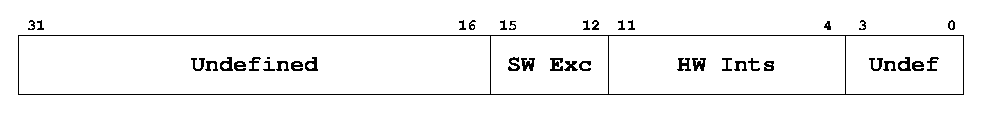
\includegraphics[width=\textwidth]{estat.eps}
\caption{\$estat - Exception Status Register}
\label{estat_pic}
\end{center}
\end{figure}

The exception status register provides the exception handler with the
ability to discover what exceptions caused it to be called. The
exception status register has a single bit flag for each external IRQ
line. Bit 4 of the status register corresponds to IRQ0, bit 5 to IRQ 1
and so on. In addition to the eight external interrupt sources the
status register also provides the status for the four CPU internal
exception sources.

The full list of all exception sources and their related status
register bit is given in Table~\ref{table:sta_loc}.

\begin{table}[h]
\begin{center}
\begin{tabular}{|l|c|}
\hline
\textbf{Exception source} & \textbf{Bit location} \\
\hline
IRQ0 & 4 \\
\hline
IRQ1 - User Interrupt Button & 5 \\
\hline
IRQ2 - Timer Interrupt & 6 \\
\hline
IRQ3 - Parallel Interrupt & 7 \\
\hline
IRQ4 - Serial Port 1 Interrupt & 8 \\
\hline
IRQ5 - Serial Port 2 Interrupt & 9 \\
\hline
IRQ6 & 10 \\
\hline
IRQ7 & 11 \\
\hline
General Protection Fault Exception & 12 \\
\hline
System Call Exception & 13 \\
\hline
Breakpoint Exception & 14 \\
\hline
Arithmetic Exception & 15 \\
\hline
\end{tabular}
\caption{Exception Status Register Fields}
\label{table:sta_loc}
\end{center}
\end{table}


\newpage
\section{Details of the Serial ports}
\label{org_sp_defn}



The REX board provides two serial interfaces, one of which is
connected to the Linux machine and the other is connected to the
terminal that should be sitting on the shelf above the board. 

For each of the serial interfaces there are 4 registers accessible to
the CPU. These registers are the transmit data register, the receive
data register, the status register and the control register.

The transmit data register holds the value that is to be sent out of
the serial port. The receive data register holds the value that has
been received in the serial port. The status register indicates if
there is a value in the receive data register and also if the value in
the transmit data register has been sent. The control register allows
the configuration of the serial port. For this Exercise the control
register will have already been configured for you by the monitor so
it will not need to be altered. Each serial port has a base address
and the 4 registers for each serial port are expressed as an offset
from this address. The base addresses for each port are defined in
table~\ref{table:serialbase} and the offsets are defined in
table~\ref{table:serialoffset}. The format of the status register for
each of the serial devices is shown in table~\ref{table:serialstat}.

\begin{table}[h]
\begin{center}
\begin{tabular}{|l|l|}
\hline
\textbf{Port} & \textbf{Base Address} \\
\hline
Linux machine & 0x70000 \\ 
\hline
Terminal & 0x71000 \\
\hline
\end{tabular}
\end{center}
\caption{Base addresses for each serial port}
\label{table:serialbase}
\end{table}

\begin{table}[h]
\begin{center}
\begin{tabular}{|l|l|}
\hline
\textbf{Register} & \textbf{Address} \\
\hline
Transmit Data & Base + 0 \\ 
\hline
Receive Data & Base + 1 \\
\hline
Control & Base + 2 \\
\hline
Status & Base + 3 \\
\hline
\end{tabular}
\end{center}
\caption{Offsets for each register}
\label{table:serialoffset}
\end{table}

\begin{table}[h]
\begin{center}
\begin{tabular}{|l|l|}
\hline
\textbf{Bit} & \textbf{Function} \\
\hline
0 & Receive Data Ready \\
 & 1 if data in receive data register, 0 otherwise \\
\hline
1 & Transmit Data Sent \\
 & 1 if ready for next character, 0 if data is still being transmitted  \\
\hline
\end{tabular}
\end{center}
\caption{Status register format}
\label{table:serialstat}
\end{table}

\subsection{Serial Control Register}

This register allows line parameters such as serial bit rate to be
set. The serial ports are configured appropriately by the monitor for
the device setup used by the Computer Systems course. Unless you know
that you specifically need to change something in this register you
should leave it as default.

The control register also controls when the serial port will cause an
interrupt. The serial port can selectively cause an interrupt when a
character is received into the receive data register, the transmit
data register becomes empty or on an error condition. Any combination of
these can be enabled or disabled at one time. To enable interrupts to
be used by the serial port under specific circumstances a `\texttt{1}'
should be written to the appropriate location. If an interrupt has
occurred it must be acknowledged by writing into the serial interrupt
acknowledge register.

The REX board monitor will initialise the serial port so that no
interrupts are enabled

The control register is a read/write register. Writes to this register
have an immediate effect on the line settings.

\begin{figure}[h]
\begin{center}
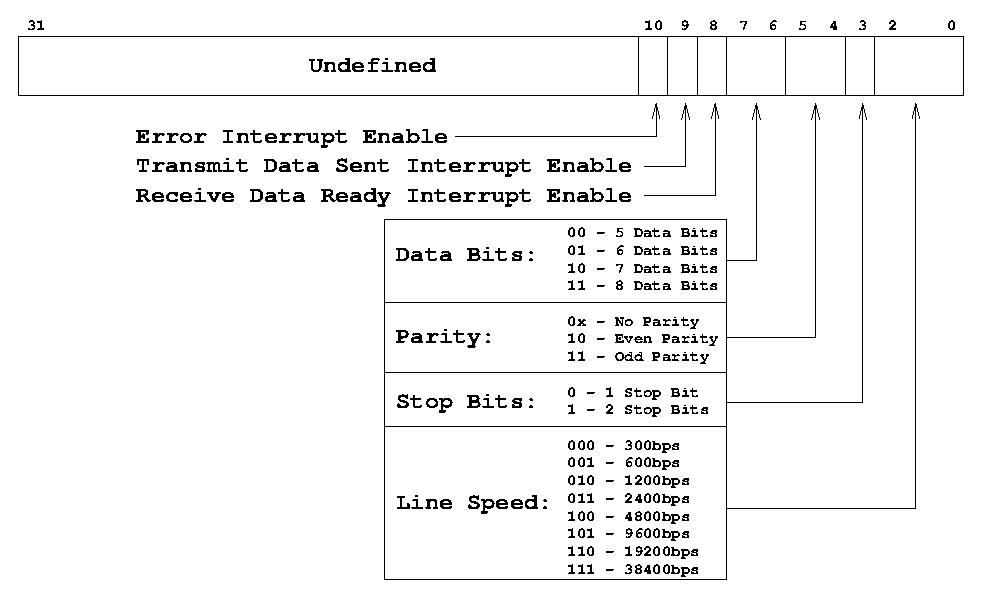
\includegraphics[width=0.8\textwidth]{serial_cr.eps}
\caption{The Serial Control Register}
\label{serial_cr_pic}
\end{center}
\end{figure}

\noindent
eg. To configure a serial interface to operate with no interrupts
enabled, at 9600 bits per second, with 8 data bits, no parity and 1
stop bit, the value `\texttt{00011000101}' would be written to the
control register.

\end{document}




